
\documentclass[12pt,a4paper]{article}

\usepackage[utf8]{inputenc}
\usepackage[T1]{fontenc}
\usepackage[brazil]{babel}
\usepackage{geometry}
\usepackage{graphicx}
\usepackage{booktabs}
\usepackage{float}
\usepackage{hyperref}
\usepackage{xcolor}
\usepackage{listings}
\usepackage{caption}
\usepackage{array}
\usepackage{mathptmx}
\usepackage{microtype}

\geometry{margin=2.5cm}
\setlength{\parindent}{0pt}
\setlength{\parskip}{0.65em}

\hypersetup{
    colorlinks=true,
    linkcolor=black,
    urlcolor=blue,
    citecolor=black
}

\lstdefinestyle{code}{
    basicstyle=\ttfamily\small,
    breaklines=true,
    frame=single,
    columns=fullflexible,
    keepspaces=true,
    backgroundcolor=\color{gray!8}
}
\lstset{style=code}

\title{Análise Global de Mudanças Climáticas com Apache Spark}
\author{Rodrigo Macedo e Gabriel Peres}
\date{2026}

\begin{document}

\maketitle

\begin{abstract}
Este relatório descreve um pipeline distribuído em Apache Spark para analisar dados climáticos e emissões de CO2. O projeto usa bases reais de temperatura global por cidade e emissões da OWID, executa limpeza, agregações, cruzamentos, funções de janela, cache, regressão com MLlib e geração de gráficos. A execução foi validada em Docker local e em dois computadores conectados por rede local, com acompanhamento pela Spark UI.
\end{abstract}

\tableofcontents
\newpage

\section{Objetivo}

Este relatório apresenta o projeto desenvolvido para o trabalho proposto pelo professor. O foco da entrega é aplicar Apache Spark em um problema real de análise de dados, mostrando leitura de bases climáticas, limpeza, transformação, cruzamento entre temperatura e CO2, execução distribuída, respostas das questões pedidas e avaliação prática de desempenho.

Este PDF é o principal material de avaliação. Por isso, ele reúne o processo completo em formato explicativo: quais dados foram usados, por que cada tratamento foi feito, onde o Spark divide o processamento, como cada pergunta foi respondida e como validamos a execução em Docker local e em dois computadores. O notebook \path{notebooks/apresentacao_spark_clima.ipynb} fica como apoio executável para demonstrar o mesmo fluxo rodando passo a passo.

\section{Arquitetura e fluxo de comunicação}

O projeto usa PySpark com DataFrames. A aplicação é empacotada em Docker para que o mesmo código rode no modo local e no modo distribuído em dois computadores. Isso reduz diferenças de ambiente e facilita repetir a execução durante a apresentação.

No modo local, o arquivo \texttt{docker-compose.yml} sobe um master Spark e dois workers no mesmo computador. Esse modo é útil para testar o pipeline inteiro sem depender de rede externa. No modo distribuído, o PC 1 roda o master, um worker local e o driver do job. O PC 2 roda outro worker apontando para o master do PC 1:

\begin{lstlisting}
spark://<IP_DO_PC_1>:7077
\end{lstlisting}

O fluxo de comunicação fica assim:

\begin{enumerate}
    \item O driver inicia o job e conversa com o master Spark.
    \item O master registra os workers disponíveis.
    \item O driver monta o plano lógico e físico das operações.
    \item O Spark quebra o plano em jobs, stages e tasks.
    \item O master agenda tasks nos executores dos workers.
    \item Os executores leem suas partições de dados, processam e devolvem resultados intermediários.
    \item O driver coleta apenas os resultados pequenos que precisam virar tabela, gráfico ou arquivo final.
\end{enumerate}

\begin{table}[H]
\centering
\caption{Componentes da arquitetura}
\begin{tabular}{p{0.25\textwidth}p{0.65\textwidth}}
\toprule
Componente & Papel no trabalho \\
\midrule
Driver & Processo que submete o job, cria a SparkSession, chama as funções do pipeline e coordena as ações. \\
Master Spark & Serviço que conhece os workers vivos e agenda recursos para os executores. \\
Worker & Processo que oferece CPU e memória para o cluster. No teste em 2 PCs, há um worker em cada máquina. \\
Executor & Processo que roda tasks Spark dentro de um worker. É nele que as partições são processadas. \\
Spark UI & Interface usada para provar visualmente workers, executores, jobs, stages, tasks e duração das etapas. \\
\bottomrule
\end{tabular}
\end{table}

\subsection{Portas usadas}

\begin{table}[H]
\centering
\caption{Portas usadas no modo distribuído}
\begin{tabular}{ll}
\toprule
Porta & Função \\
\midrule
7077 & Master Spark, usado pelos workers para conexão. \\
8080 & Spark UI do master, usada para mostrar os workers vivos. \\
40444 & Porta do driver do job. \\
40445 & Block manager, usado em comunicação de blocos e dados intermediários. \\
\bottomrule
\end{tabular}
\end{table}

\subsection{Decisões de arquitetura}

A primeira decisão foi manter os dados replicados nos dois computadores no modo \texttt{raw}. Cada executor lê arquivos locais montados em \texttt{/app/data/...}. Isso evita depender de HDFS, S3 ou outro storage distribuído, que aumentaria o escopo do trabalho. A consequência é que PC 1 e PC 2 precisam ter o mesmo diretório \texttt{data/raw} antes do benchmark.

A segunda decisão foi usar DataFrames em vez de RDDs manuais. DataFrames permitem que o Catalyst otimize filtros, agregações, joins e projeções. Para este trabalho, isso é mais adequado porque as perguntas são consultas analíticas sobre tabelas.

A terceira decisão foi salvar saídas pequenas em \texttt{output/results} e gráficos em \texttt{output/plots}. O processamento pesado fica no Spark. A conversão para pandas só acontece depois que os dados já foram agregados e estão pequenos o bastante para caber no driver.

\section{Bases usadas}

Foram usadas duas fontes principais:

\begin{itemize}
    \item Temperatura: Berkeley Earth, arquivo \texttt{GlobalLandTemperaturesByCity.csv}.
    \item CO2: OWID, arquivo \texttt{owid-co2-data.csv}.
\end{itemize}

O arquivo \texttt{GlobalTemperatures.csv} também fica disponível no projeto, mas a resposta da questão sobre zonas tropicais usa a base por cidade, porque ela contém cidade, país, latitude e longitude. Essa escolha permite filtrar regiões tropicais diretamente pela latitude.

\section{Fluxo do pipeline}

O pipeline segue a ordem abaixo:

\begin{enumerate}
    \item Ler os CSVs com Spark.
    \item Limpar a base de temperatura.
    \item Limpar a base de CO2.
    \item Criar colunas auxiliares como ano, mês, década e país normalizado.
    \item Agregar temperatura mensal por cidade para temperatura anual por país.
    \item Cruzar temperatura e CO2 por país e ano.
    \item Responder as perguntas com agregações, joins, window functions e MLlib.
    \item Gerar tabelas, gráficos e arquivos de saída.
\end{enumerate}

\subsection{Limpeza de temperatura}

A limpeza remove registros sem \texttt{AverageTemperature}, converte \texttt{dt} para data, extrai \texttt{year}, \texttt{month} e \texttt{decade}, converte coordenadas como \texttt{23.55S} para valores numéricos negativos e remove temperaturas fora de \texttt{-90 C} a \texttt{70 C}. Esse limite é uma regra de sanidade: ele não pretende modelar clima, apenas evita que erro de leitura ou valor impossível distorça médias e desvios.

Também é criada a coluna \texttt{country\_norm}. Ela normaliza o nome do país para permitir o join com CO2. Sem essa coluna, diferenças pequenas de caixa, espaço ou acento poderiam impedir cruzamentos corretos.

\subsection{Limpeza de CO2}

A base de CO2 passa por filtros para remover agregados como \texttt{World}, \texttt{Asia} e \texttt{Europe}. Esses registros não representam países e poderiam duplicar a escala da análise. Também são mantidos apenas anos a partir de 1900 e linhas com \texttt{co2} preenchido.

A mesma regra de \texttt{country\_norm} é aplicada. Isso garante que o join use a mesma chave nas duas bases.

\subsection{Cruzamento dos dados}

Antes do join, a temperatura mensal por cidade é agregada para temperatura anual por país:

\begin{lstlisting}
country_norm + year -> avg_temperature
\end{lstlisting}

Depois disso, o join com CO2 usa:

\begin{lstlisting}
country_norm + year
\end{lstlisting}

Essa transformação muda a granularidade dos dados. A temperatura começa mensal e por cidade. O CO2 está anual e por país. Para cruzar as bases, as duas precisam chegar ao mesmo nível: país e ano.

\section{Respostas das questões}

\subsection{Questão 1: média anual global por década}

Primeiro calculamos a média anual global. Depois agrupamos os anos por década e aplicamos uma média móvel. A década reduz ruído anual. A média móvel ajuda a enxergar a tendência sem depender de um único ano muito frio ou muito quente.

\begin{table}[H]
\centering
\caption{Média anual global por década}
\begin{tabular}{rrr}
\toprule
Década & Média anual & Média móvel \\
\midrule
1980 & 17.9578 & 17.8420 \\
1990 & 18.2497 & 18.0012 \\
2000 & 18.5268 & 18.2448 \\
2010 & 18.6335 & 18.4700 \\
\bottomrule
\end{tabular}
\end{table}

\begin{figure}[H]
\centering
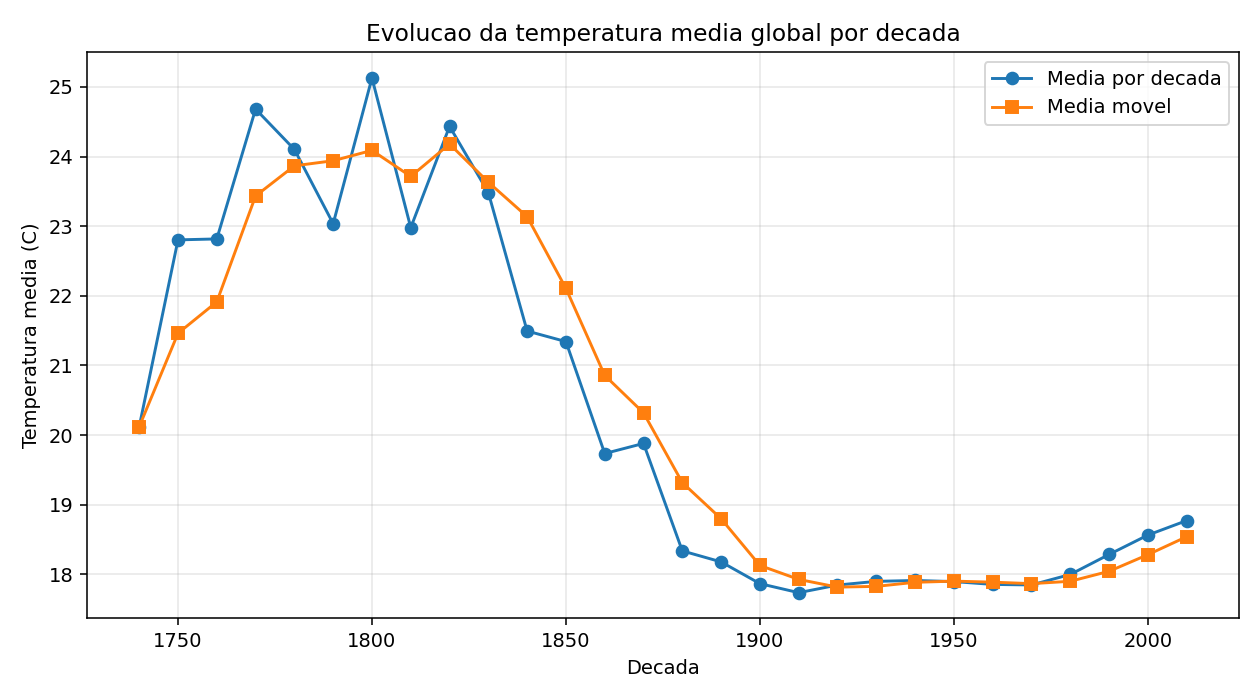
\includegraphics[width=0.92\textwidth]{figures/global_decade_temperature.png}
\caption{Evolução da temperatura média global por década.}
\end{figure}

O resultado mostra aumento nas décadas recentes. A leitura correta é de tendência agregada, não de previsão climática completa.

\subsection{Questão 2: anos mais quentes por continente}

A base original não vem com continente. Por isso, o pipeline usa um mapeamento de país para continente. Depois agrega temperatura por continente e ano, e usa \texttt{row\_number()} para escolher o ano mais quente de cada continente.

A função de ranking é importante porque evita escolher apenas o maior valor global. Cada continente precisa ter seu próprio primeiro lugar.

\begin{table}[H]
\centering
\caption{Ano mais quente por continente}
\begin{tabular}{lrr}
\toprule
Continente & Ano mais quente & Média \\
\midrule
Africa & 2010 & 24.1887 \\
Asia & 2013 & 21.3166 \\
Europe & 2007 & 9.9243 \\
North America & 2013 & 18.2733 \\
Oceania & 1998 & 16.3499 \\
South America & 2002 & 21.9883 \\
\bottomrule
\end{tabular}
\end{table}

A decisão arbitrária aqui é depender do mapeamento disponível de país para continente. Se um país não estiver mapeado, ele fica fora desse recorte. Isso muda a cobertura, mas mantém a pergunta tecnicamente correta para os países classificados.

\subsection{Questão 3: cidades em risco}

O critério do enunciado é o desvio padrão de temperatura. Por isso, a pergunta não mede maior aquecimento médio, e sim maior variação histórica de temperatura. As cidades no topo aparecem em regiões continentais frias, onde a amplitude sazonal costuma ser alta.

\begin{table}[H]
\centering
\caption{Cidades com maior desvio padrão}
\begin{tabular}{llr}
\toprule
Cidade & País & Desvio padrão \\
\midrule
Heihe & Russia & 16.4134 \\
Blagoveshchensk & Russia & 16.4134 \\
Kyzyl & Russia & 16.3454 \\
Hailar & China & 16.3026 \\
Yakeshi & China & 16.3026 \\
\bottomrule
\end{tabular}
\end{table}

Esse resultado deve ser explicado com cuidado: alto desvio padrão indica grande oscilação, não necessariamente a maior alta recente de temperatura. Se o critério mudasse para crescimento por década, o ranking poderia mudar.

\subsection{Questão 4: correlação entre mínima e máxima em zonas tropicais}

A base por cidade não possui colunas reais de mínima e máxima. Para responder mantendo o foco em zonas tropicais, filtramos cidades entre \texttt{-23.5} e \texttt{23.5} de latitude. Depois, para cada cidade e ano, usamos uma aproximação:

\begin{itemize}
    \item mínima anual aproximada: menor média mensal do ano;
    \item máxima anual aproximada: maior média mensal do ano.
\end{itemize}

Essa é a principal limitação da questão. O cálculo não usa mínima e máxima meteorológicas reais, e sim extremos entre médias mensais. A vantagem é que a resposta fica compatível com a base disponível. A diferença prática é que extremos diários são suavizados, então a correlação tende a representar comportamento anual agregado.

O Pearson encontrado foi:

\begin{lstlisting}
0.4220268963949332
\end{lstlisting}

Isso indica correlação positiva moderada entre os meses mais frios e mais quentes nas cidades tropicais.

\subsection{Questão 5: qualidade dos dados}

A pergunta usa a incerteza da temperatura. A regra aplicada foi:

\begin{lstlisting}
AverageTemperatureUncertainty > 0.10 * abs(media_historica_da_cidade)
\end{lstlisting}

O percentual de 10\% é um corte definido para separar registros mais instáveis. Se esse percentual for reduzido, mais registros entram como alta incerteza. Se for aumentado, menos registros são marcados. Por isso, o notebook deixa essa variável fácil de alterar durante a apresentação.

\begin{table}[H]
\centering
\caption{Registros com alta incerteza}
\begin{tabular}{lr}
\toprule
Alta incerteza & Registros \\
\midrule
true & 1.608.419 \\
false & 6.626.663 \\
\bottomrule
\end{tabular}
\end{table}

A marcação de incerteza não remove os dados automaticamente. Ela cria uma coluna de qualidade para análise e discussão.

\subsection{Questão 6: aumento de CO2 versus aumento de temperatura}

Para cada país nos últimos 50 anos disponíveis, capturamos o primeiro e o último ano do período. Depois calculamos:

\begin{lstlisting}
co2_delta = co2_final - co2_inicial
temp_delta = temp_final - temp_inicial
\end{lstlisting}

O Pearson entre os deltas foi:

\begin{lstlisting}
0.07968357901250334
\end{lstlisting}

\begin{figure}[H]
\centering
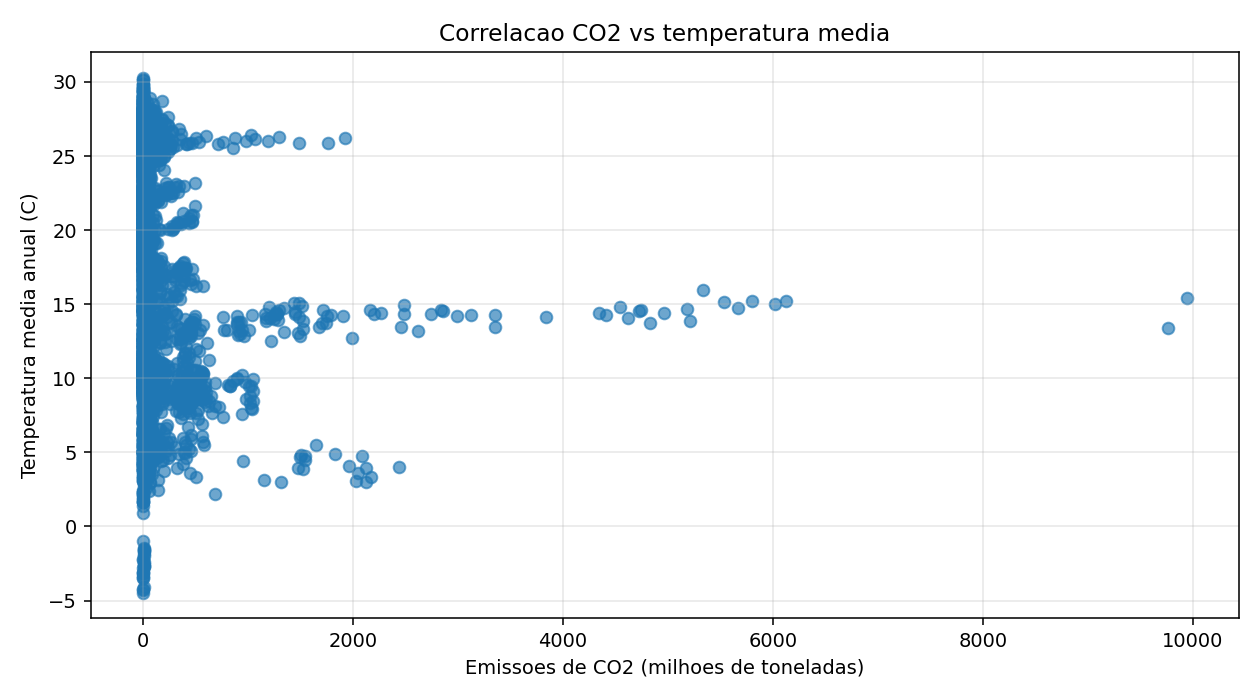
\includegraphics[width=0.92\textwidth]{figures/co2_temperature_scatter.png}
\caption{Dispersão entre variação de CO2 e variação de temperatura.}
\end{figure}

A correlação ficou fraca. Isso não invalida o processamento. A pergunta cruza duas bases reais e calcula uma relação estatística simples. A limitação é de interpretação: emissões absolutas por país misturam população, economia, matriz energética, latitude, território e geografia. Isso mede associação no recorte escolhido, não causalidade climática.

\subsection{Questão 7: ranking de aceleração térmica}

A questão usa window functions com \texttt{lag} por país. Primeiro calculamos médias por década. Depois comparamos a última década completa com a anterior. Como a base Berkeley termina por volta de 2013, a última década completa usada foi \texttt{2000-2009}.

\begin{table}[H]
\centering
\caption{Países com maior aceleração térmica}
\begin{tabular}{lrr}
\toprule
País & Década & Aceleração \\
\midrule
Azerbaijan & 2000 & 0.4929 \\
Kazakhstan & 2000 & 0.4900 \\
Uzbekistan & 2000 & 0.4680 \\
Tajikistan & 2000 & 0.4657 \\
Afghanistan & 2000 & 0.4562 \\
\bottomrule
\end{tabular}
\end{table}

A decisão de usar apenas décadas completas evita comparar uma década cheia com uma década parcial. Se usássemos 2010-2013, a comparação poderia ficar artificial porque o período teria menos anos.

\subsection{Questão 8: previsão com MLlib}

Foi usado \texttt{LinearRegression} do Spark MLlib. A feature é o ano e o label é a temperatura média. Para \texttt{Rio De Janeiro, Brazil}, a base termina antes dos anos atuais. Por isso, os cinco anos previstos são os cinco anos seguintes ao último ano disponível.

\begin{table}[H]
\centering
\caption{Previsão para Rio de Janeiro}
\begin{tabular}{rr}
\toprule
Ano & Temperatura prevista \\
\midrule
2014 & 20.5780 \\
2015 & 20.5762 \\
2016 & 20.5745 \\
2017 & 20.5727 \\
2018 & 20.5710 \\
\bottomrule
\end{tabular}
\end{table}

\begin{figure}[H]
\centering
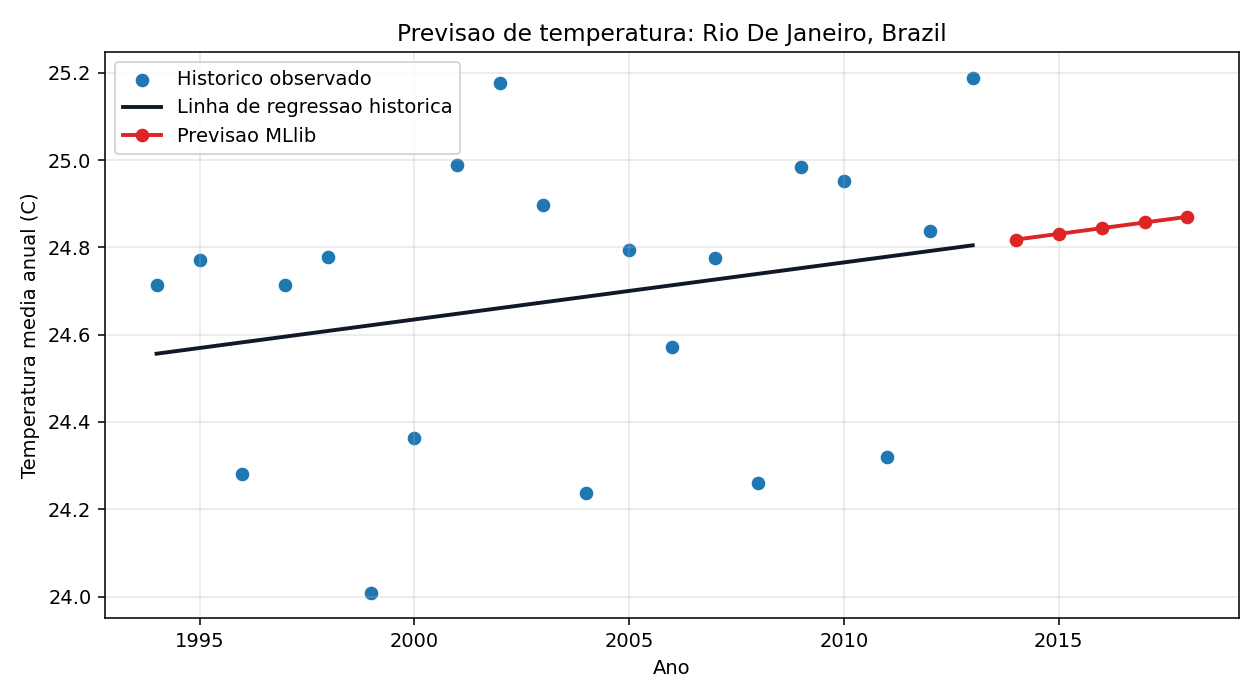
\includegraphics[width=0.92\textwidth]{figures/temperature_forecast_Rio_De_Janeiro_Brazil.png}
\caption{Previsão para Rio de Janeiro. Os pontos históricos não são conectados; a linha mostra a regressão e a projeção.}
\end{figure}

A regressão linear foi escolhida por ser simples de explicar e por existir no MLlib. Ela não pretende ser o melhor modelo climático possível. Se fossem usados mais atributos, como CO2, latitude, sazonalidade ou janelas temporais, a modelagem mudaria. Aqui o objetivo é mostrar o uso de MLlib no pipeline distribuído.

\section{Spark, paralelismo e conclusão prática}

Esta seção junta a leitura técnica do Spark com as medições feitas no projeto. Ela é a parte mais importante para defender que o trabalho distribui processamento, mas também para explicar por que distribuir não significa automaticamente reduzir tempo.

\subsection{Onde o Spark divide o trabalho}

A divisão acontece nas partições dos DataFrames. Quando o Spark lê arquivos CSV, ele cria partições. Operações como \texttt{groupBy}, \texttt{join}, \texttt{orderBy} e window functions geram stages e tasks. Cada task pode ser enviada para um executor disponível.

Na Spark UI, essa divisão aparece em:

\begin{itemize}
    \item \textbf{Workers}: máquinas conectadas ao master.
    \item \textbf{Executors}: processos que executam tasks.
    \item \textbf{Jobs}: ações disparadas pelo código, como \texttt{collect}, \texttt{count} e escrita de arquivos.
    \item \textbf{Stages}: partes do plano separadas por shuffle.
    \item \textbf{Tasks}: menor unidade de execução distribuída.
\end{itemize}

Ver dois workers vivos na Spark UI confirma que o cluster está conectado. Para confirmar que o job usou os dois, também é preciso olhar executors, hosts, tasks e tempo de execução durante a rodada.

\subsection{Cache e reaproveitamento de etapas}

O modo \texttt{--cache on} persiste DataFrames reutilizados:

\begin{itemize}
    \item temperatura limpa;
    \item CO2 limpo;
    \item temperatura anual por país;
    \item temperatura anual por cidade;
    \item join entre temperatura e CO2.
\end{itemize}

O cache é útil porque várias perguntas usam as mesmas bases intermediárias. Sem cache, o Spark pode recomputar leitura, limpeza e agregações várias vezes.

\begin{table}[H]
\centering
\caption{Tempo por pergunta com e sem cache}
\begin{tabular}{lrrr}
\toprule
Pergunta & Com cache (s) & Sem cache (s) & Ganho aproximado \\
\midrule
Q1 & 2.3362 & 5.5426 & 2.37x \\
Q2 & 3.9009 & 12.3879 & 3.18x \\
Q3 & 1.7852 & 12.7051 & 7.12x \\
Q4 & 2.4746 & 12.0828 & 4.88x \\
Q5 & 0.9610 & 14.3473 & 14.93x \\
Q6 & 0.6194 & 14.3876 & 23.23x \\
Q7 & 4.3224 & 24.9529 & 5.77x \\
Q8 & 3.9533 & 22.0286 & 5.57x \\
\midrule
Total & 20.3530 & 118.4348 & 5.82x \\
\bottomrule
\end{tabular}
\end{table}

\begin{figure}[H]
\centering
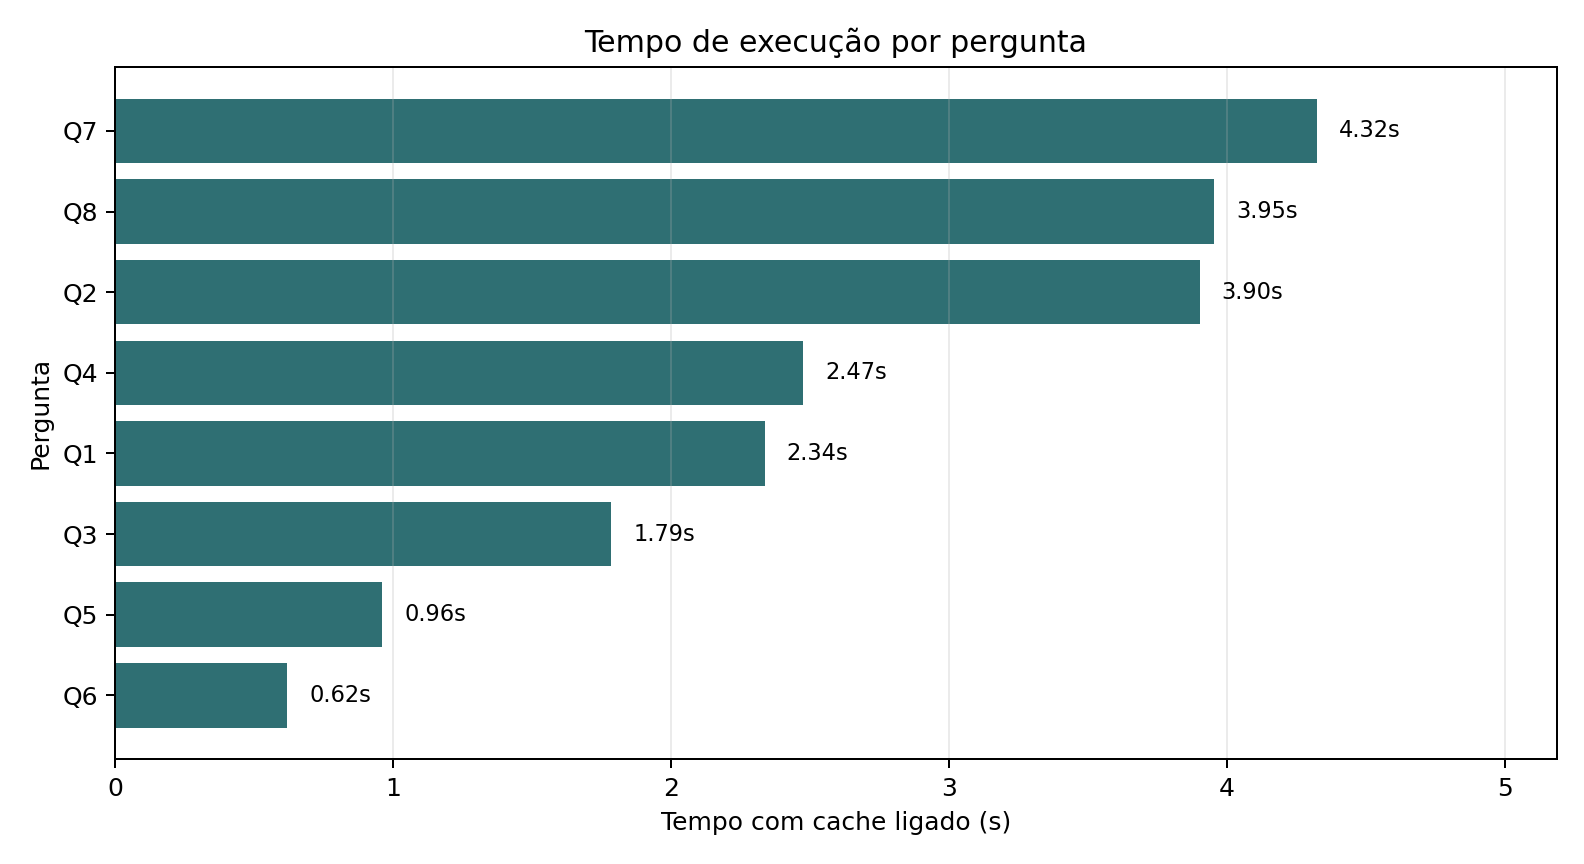
\includegraphics[width=0.92\textwidth]{figures/timings_cache_on_barh.png}
\caption{Tempo das perguntas com cache ligado. Os rótulos foram reduzidos para Q1 a Q8 para facilitar a leitura.}
\end{figure}

O maior ganho aparece nas perguntas que reutilizam bases limpas e joins. A Q6, por exemplo, depende do cruzamento entre temperatura e CO2. Com cache, o Spark reaproveita o resultado intermediário; sem cache, precisa refazer mais trabalho.

\subsection{Benchmark local versus cluster LAN}

A configuração principal do trabalho usa dois workers. No Compose local, os dois workers ficam no PC 1. No cluster LAN, um worker fica no PC 1 e outro no PC 2. O script \path{scripts/benchmark_cluster_modes.sh} mede tempo total, tempo de processamento Spark e overhead aproximado.

\begin{table}[H]
\centering
\caption{Comparação entre execução local e cluster LAN}
\small
\begin{tabular}{p{0.22\textwidth}p{0.28\textwidth}rrr}
\toprule
Modo & Workers & Wall (s) & Spark (s) & Overhead (s) \\
\midrule
local-compose & 2 workers no PC 1 & 158 & 35.4613 & 122.5387 \\
lan-cluster & 1 worker no PC 1 e 1 no PC 2 & 188 & 43.8593 & 144.1407 \\
\bottomrule
\end{tabular}
\normalsize
\end{table}

O modo local foi mais rápido nesta carga. O modo LAN distribuiu o processamento entre dois computadores, mas teve overhead maior.

Com esses valores:

\begin{lstlisting}
speedup_lan_vs_local = 158 / 188 = 0.84
eficiencia_lan = 0.84 / 2 = 0.42
diferenca_de_overhead = 144.1407 - 122.5387 = 21.6020s
\end{lstlisting}

A conclusão prática é que o processamento foi distribuído, mas esta execução em LAN não foi mais rápida. A Spark UI confirmou dois workers vivos e executores em hosts diferentes. Mesmo assim, o custo de rede, Docker, submit, shuffle e sincronização superou o ganho de usar o PC 2.

\subsection{Workers, recursos e escalabilidade}

Os workers locais usam:

\begin{lstlisting}
--cores 2
--memory 2G
\end{lstlisting}

Para testar mais recursos por worker, pode-se mudar para:

\begin{lstlisting}
--cores 4
--memory 4G
\end{lstlisting}

Isso só faz sentido se a máquina tiver CPU e memória disponíveis. Mais recursos não garantem melhora se o gargalo estiver em leitura de disco, shuffle, driver, escrita final ou etapas pouco paralelizáveis.

No Compose atual, os workers estão nomeados como \texttt{spark-worker-1} e \texttt{spark-worker-2}. Para três workers, duplica-se o bloco e cria-se \texttt{spark-worker-3}, com porta \texttt{8083:8081}. Para quatro workers, cria-se \texttt{spark-worker-4}, com porta \texttt{8084:8081}.

Se o Compose for refatorado para um serviço genérico \texttt{spark-worker}, a escala poderia ser feita com:

\begin{lstlisting}
SPARK_WORKER_CORES=2 SPARK_WORKER_MEMORY=2G docker compose up -d --scale spark-worker=3
SPARK_WORKER_CORES=2 SPARK_WORKER_MEMORY=2G docker compose up -d --scale spark-worker=4
\end{lstlisting}

Para comparar N workers contra a base de dois workers:

\begin{lstlisting}
speedup = tempo_2_workers / tempo_N_workers
eficiencia = speedup / (N / 2)
constante_de_rede_aproximada = network_orchestration_overhead
\end{lstlisting}

Os testes com três e quatro workers são uma extensão natural do experimento, mas não fazem parte da medição principal registrada aqui.

\subsection{Por que mais workers podem não reduzir o tempo}

Se três ou quatro workers não diminuírem o tempo, os motivos mais prováveis são:

\begin{itemize}
    \item dataset pequeno para o custo de distribuir;
    \item poucas partições;
    \item workers no mesmo PC competindo pelo mesmo disco;
    \item shuffle alto;
    \item escrita final serializada por \texttt{coalesce(1)};
    \item driver virando gargalo;
    \item etapas com window functions sem \texttt{partitionBy};
    \item custo de rede maior que o ganho de paralelismo.
\end{itemize}

Durante a execução apareceu o aviso:

\begin{lstlisting}
WindowExec: No Partition Defined for Window operation
\end{lstlisting}

Isso indica que algumas janelas foram executadas sem particionamento explícito, fazendo o Spark mover dados para uma única partição. Esse trecho reduz o paralelismo e ajuda a explicar por que o ganho não é linear.

\subsection{Conclusão a partir das medições}

O projeto demonstra um pipeline Spark completo e distribuído: leitura de CSVs reais, limpeza, normalização, agregações, join entre temperatura e CO2, window functions, cache, MLlib, escrita de resultados e geração de gráficos.

A execução em dois PCs foi validada pela Spark UI com dois workers vivos e executores em hosts diferentes. A medição com base \texttt{raw} mostrou que distribuir não garante acelerar sempre. O Compose local terminou em 158 segundos, enquanto o cluster LAN terminou em 188 segundos. O modo LAN teve 21.6020 segundos a mais de overhead estimado.

A parte mais favorável do pipeline foi o cache: nas perguntas Q1 a Q8, o tempo somado caiu de 118.4348 segundos sem cache para 20.3530 segundos com cache, um ganho aproximado de 5.82x. Isso mostra que, para este trabalho, reaproveitar etapas intermediárias foi mais impactante do que apenas adicionar outro computador.

Portanto, a defesa técnica é: o cluster funcionou, os dados e o processamento foram distribuídos, mas o ganho de desempenho depende do tamanho da carga, do número de partições, do custo de shuffle, da rede e das partes serializadas do pipeline.

\end{document}
